\documentclass[dvipdfmx,autodetect-engine]{jsarticle}
\usepackage[utf8]{inputenc}
\usepackage{graphicx}
\usepackage{color}
\usepackage{amsmath}
\usepackage{braket}%dirac notation
\usepackage{qcircuit} 
\usepackage{wrapfig}
\usepackage{fancyhdr}
\usepackage{amsmath}
\usepackage{amsfonts}
\usepackage{amssymb}
\usepackage{ascmac}
\usepackage{mathrsfs}
\usepackage{ulem}%文字に下線を引く

\usepackage{tikz}
\usetikzlibrary{arrows,decorations.markings}




\newcommand{\R}{\mathrm{R}}
\newcommand{\A}{\mathrm{A}}
\newcommand{\E}{\mathrm{E}}
\newcommand{\I}{\mathrm{I}}
\newcommand{\rL}{\mathrm{L}}
\newcommand{\C}{\mathrm{C}}
\newcommand{\J}{\mathrm{J}}
\newcommand{\rS}{\mathrm{S}}
\newcommand{\rr}{\mathrm{r}}
\newcommand{\bk}{\bm{k}}
\newcommand{\bq}{\bm{q}}
\newcommand{\bp}{\bm{p}}
\newcommand{\br}{\bm{r}}
\newcommand{\bR}{\bm{R}}

\usepackage{amsmath,amsfonts,amssymb}
\usepackage{graphicx}
\usepackage[dvipdfmx]{hyperref}
\usepackage{pxjahyper}%these two come together
\usepackage[dvipdfmx]{color}
\usepackage{braket}%dirac notation
\usepackage{wrapfig}
\usepackage{here}
\usepackage{tabularx, dcolumn}
\usepackage{subfigure}
\usepackage{cases}
\usepackage{bigints}%インテグラルで大きくする
\usepackage{mathtools} 
\hypersetup{hidelinks}
\interfootnotelinepenalty=10000 % this is to keep a footnote in a single page
\usepackage{bm}%ベクトル記号
\usepackage{ascmac} %囲い
%%%%%%
\usepackage{tikz}
\usepackage{amsmath}
\usepackage{cases}%連立方程式


%%%%%%newcomand
\newcommand{\be}{\begin{equation}}
\newcommand{\ee}{\end{equation}}
\newcommand{\nn}{\notag \\}

%operator
\newcommand{\hH}{{\hat{H}}}%ハミルトニアン
\newcommand{\hHt}{{\hat{\mathcal{H}}}}%ハミルトニアン
\newcommand{\hU}{{\hat{U}}}
\newcommand{\hM}{{\hat{M}}}
\newcommand{\hN}{{\hat{N}}}
\newcommand{\hA}{{\hat{A}}}
\newcommand{\hB}{{\hat{B}}}
\newcommand{\hO}{{\hat{O}}}
\newcommand{\hAd}{{\hat{A}^\dag}}
\newcommand{\ha}{{\hat{a}}}
\newcommand{\hb}{{\hat{b}}}
\newcommand{\had}{{\hat{a}^\dag}}
\newcommand{\hpsi}{{\hat{\psi}}}
\newcommand{\hpsid}{{\hat{\psi}^\dag}}
\newcommand{\hrho}{{\hat{\rho}}}
\newcommand{\hsig}{{\hat{\sigma}}}
\newcommand{\hx}{{\hat{x}}}
\newcommand{\hy}{{\hat{y}}}
\newcommand{\hz}{{\hat{z}}}
\newcommand{\hX}{{\hat{X}}}
\newcommand{\hY}{{\hat{Y}}}
\newcommand{\hZ}{{\hat{Z}}}
\newcommand{\hp}{{\hat{p}}}
\newcommand{\hvp}{{\hat{\bm p}}}

%\vector
\newcommand{\vr}{{\bm{r}}} %vector r
\newcommand{\vP}{{\bm{P}}} %vector r
\newcommand{\vphi}{{\varphi(t,\bm{r})}}

%

\newcommand{\tr}{\mathrm{Tr}}
\newcommand{\diag}{\mathrm{diag}}
\newcommand{\rint}{\mathrm{int}}
\newcommand{\tot}{\mathrm{tot}}


\newcommand{\KM}[1]{\textcolor[rgb]{0.1, 0.1, 1}{1}}
\newcommand{\KMdel}[1]{\textcolor[rgb]{0.1, 0.1, 0.9}{\sout{\textcolor{black}{1}}}}


\makeatletter
\title{Kitaev spin liquid}



\begin{document}
\maketitle


\tableofcontents
%目の保護用
%\pagecolor{black}
%\color{white}
%%%%%%%%%%%%%%%%%%%%%
\section*{16th, September, 2022}
\section{introduction}
この講義では,Kitaevスピン液体について学ぶ\cite{kitaev2006anyons}.
Kitaevスピン液体を通じて,量子スピン液体の性質を理解し,その量子情報操作への応用がどのようになされるか具体的に理解する.
\begin{figure}[h]
		\centering
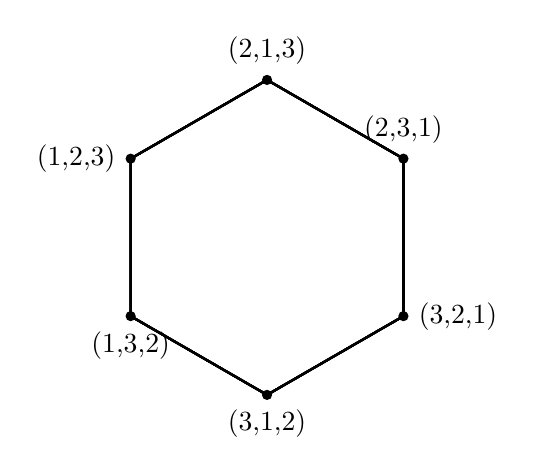
\begin{tikzpicture}
    [thick
  ,decoration =
    {markings
    ,mark=at position 0.5 with {\arrow{stealth'}}
    }
  ]
   \newdimen\R
   \R=2.0cm
   \foreach \x/\l in
    { 60/a,
     90/b,
     150/c,
     210/d,
     270/e,
     330/f
    }
   \draw  (30:\R) \foreach \x in {90,150,...,450} {  -- (\x:\R) };
   %\draw[postaction={decorate}] ({\x-60}:\R) -- node[auto,swap]{\l} (\x:\R);
   \foreach \x/\l/\p in
     { 30/{(2,3,1)}/above,
      90/{(2,1,3)}/above,
      150/{(1,2,3)}/left,
      210/{(1,3,2)}/below,
      270/{(3,1,2)}/below,
      330/{(3,2,1)}/right
     }
     \node[inner sep=1pt,circle,draw,fill,label={\p:\l}] at (\x:\R) {};
\end{tikzpicture}
		\caption{六角格子をtexで書く練習
	}
		\label{fig:swap}
	\end{figure}


\section{Kitaev model}
\begin{figure}[h]
\centering
		%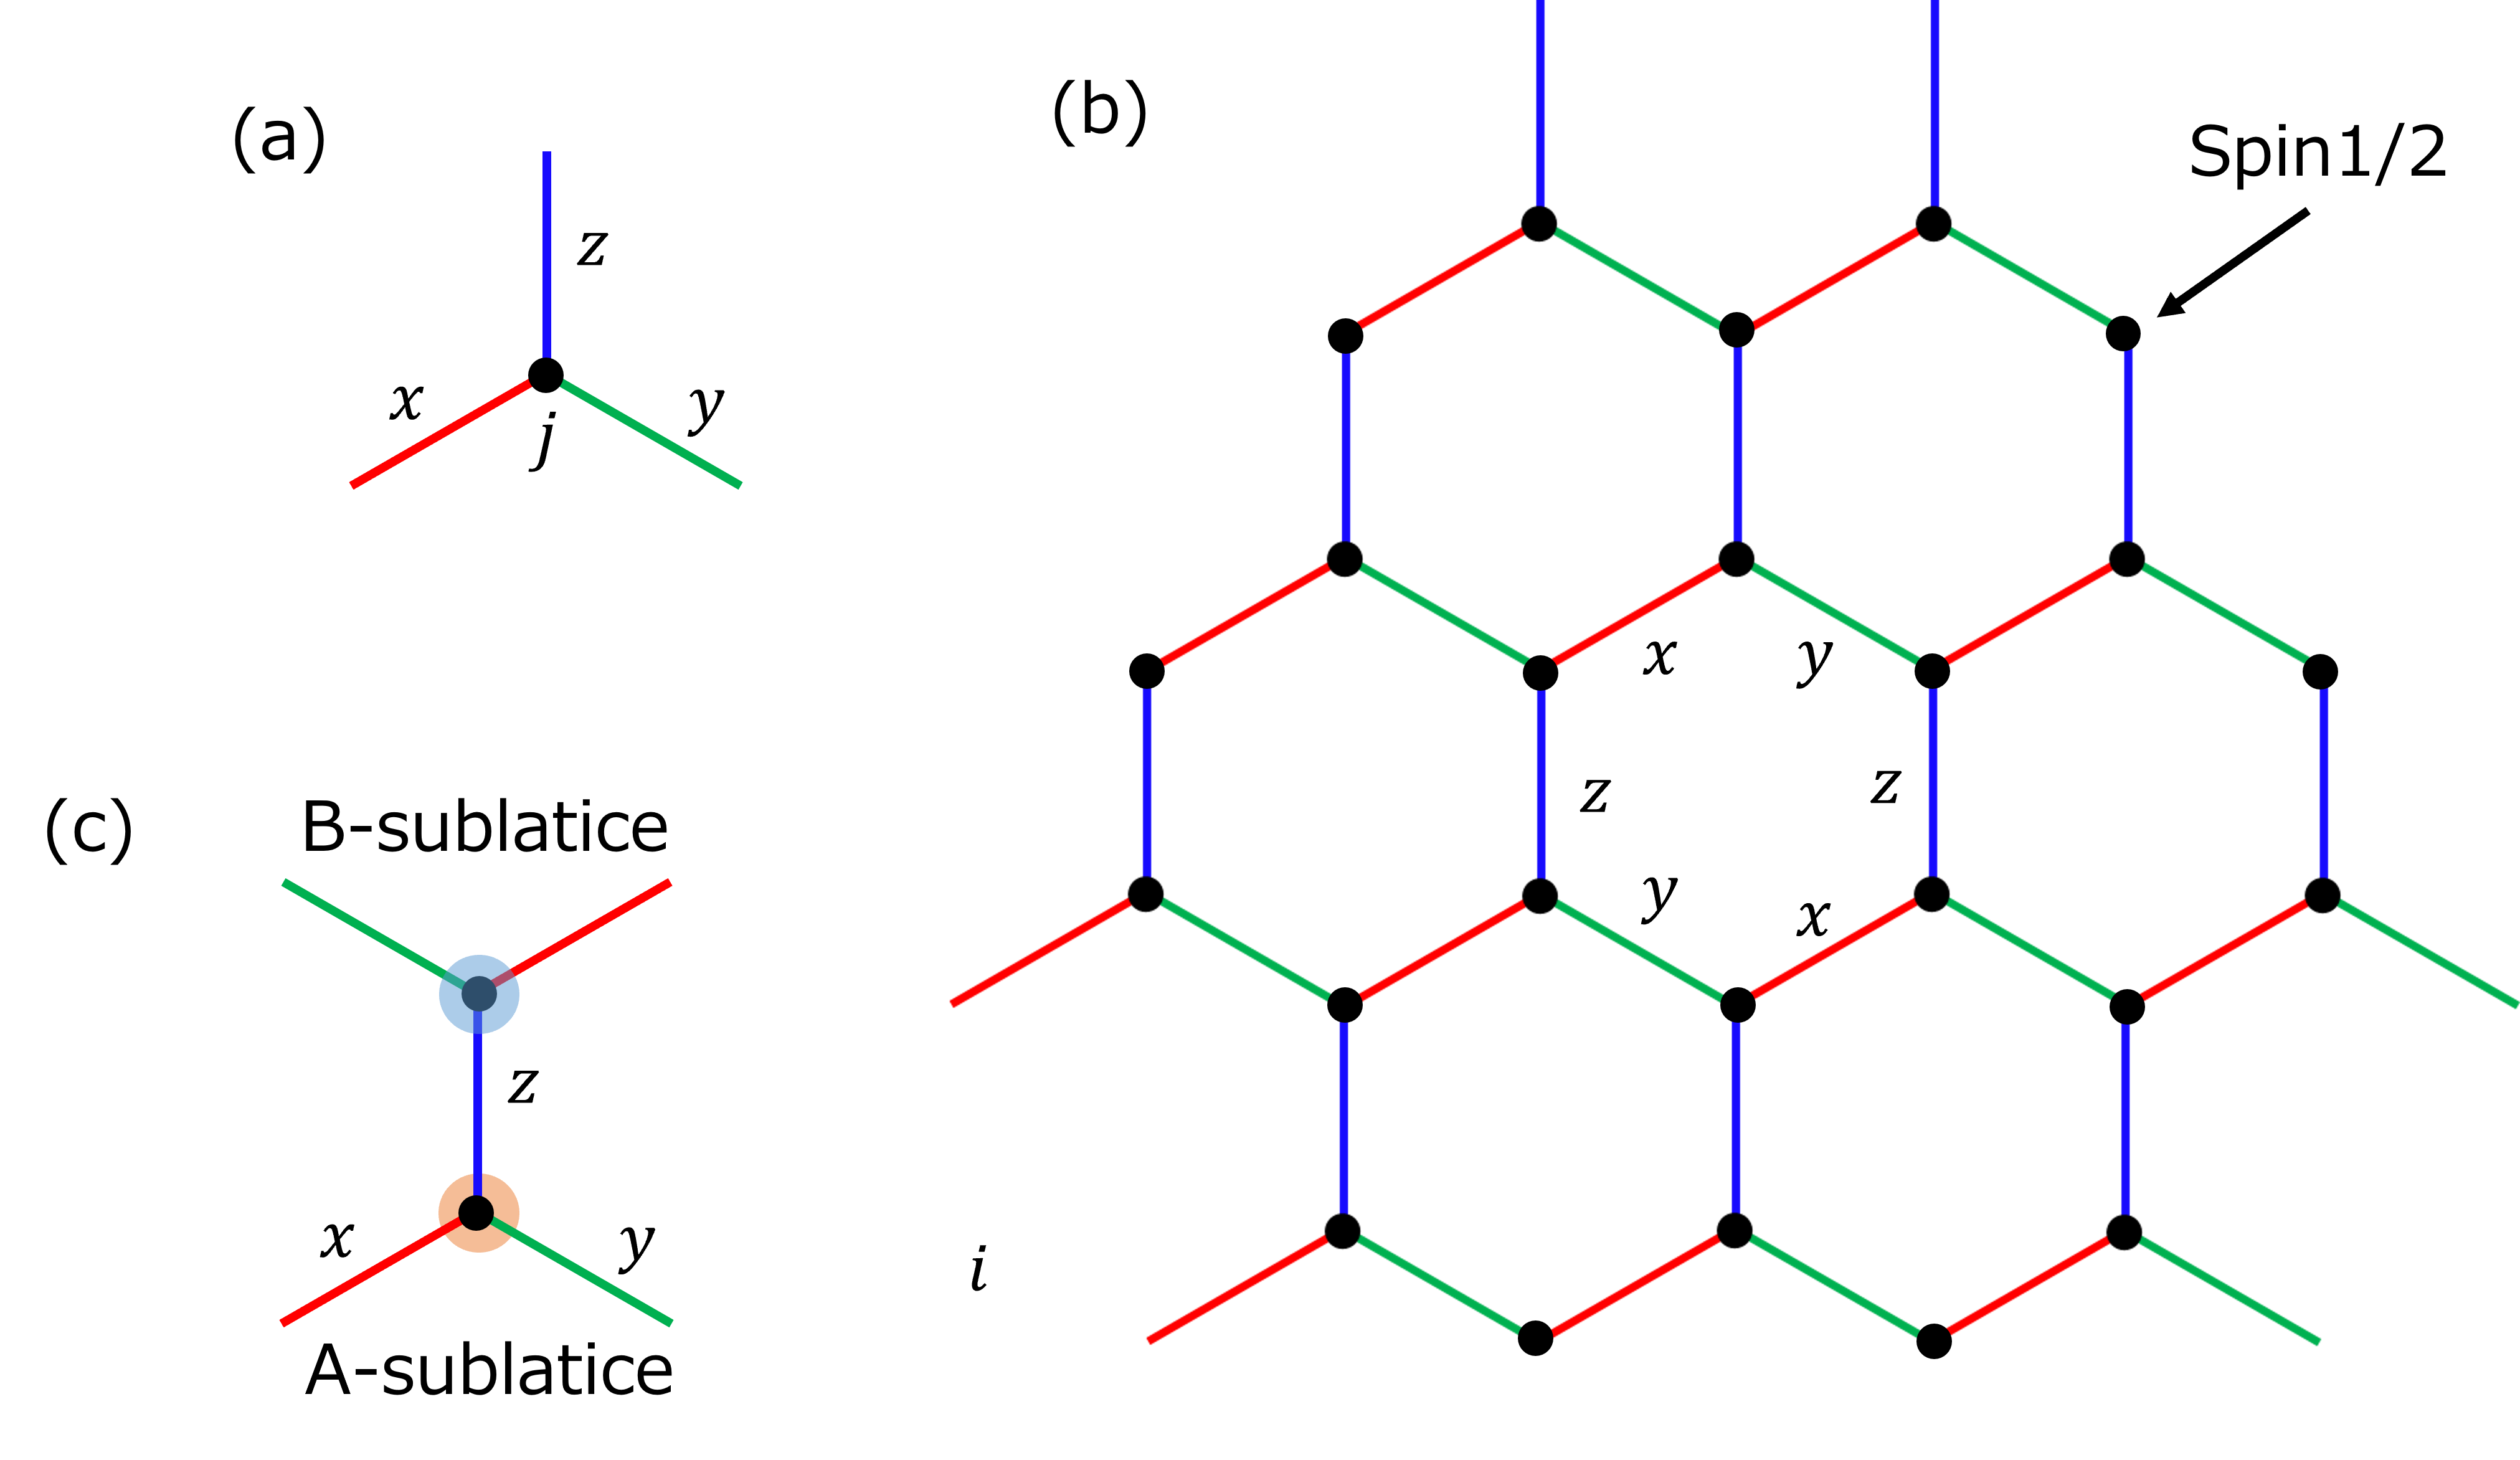
\includegraphics[width=15.0cm]{fig_kitaev/kitaevmodel.png} \\
\caption{(a)サイト$j$に対する結合.赤,緑,青はそれぞれ,$x$, $y$, $z$-interactionを表している.(b)Kitaev 模型を定義する六角格子 (honeycomb lattice).
(c)副格子.下をA-副格子,上をb-副格子と呼び,A-副格子のサイトに対応するindexを$i$とする.}
\label{fig:schematic1}
\end{figure}
\begin{equation}\label{kitaev_Hamiltonian}
    \hat{H} = -J_x\sum_{\braket{j,j^\prime}_x}\hat{S}^{x}_{j}\hat{S}^{x}_{j^\prime}
    -J_y\sum_{\braket{j,j^\prime}_y}\hat{S}^{y}_{j}\hat{S}^{y}_{j^\prime}
    -J_z\sum_{\braket{j,j^\prime}_z}\hat{S}^{z}_{j}\hat{S}^{z}_{j^\prime}
\end{equation}
ここで,$\hat{S}^{\alpha}_{j}$はサイト$j$に作用するスピン$1/2$の演算子を表す.また,$\braket{j,j^\prime}_\alpha$は$\alpha$-bondで結合するサイト$\braket{j,j^\prime}$の組を表す.例えば,サイト$j$と$j^{\prime}$とが$\hat{S}^{x}_{j}\hat{S}^{x}_{j^\prime}$ interaction;\textcolor{red}{$-$}で繋がっていれば,$\braket{j,j^\prime}_x$となる.$y$, $z$の場合も同様にして,$\braket{j,j^\prime}_y$:\textcolor{green}{$-$}, $\braket{j,j^\prime}_z$:\textcolor{blue}{$-$}と対応する.

さらにいくつかの記号を導入する.$j_\alpha$, $\alpha=\{x,y,z\}$はサイト$j$から$\alpha$-bondでつながったサイトを表す.

\subsection{マヨナラ表現}
\subsubsection{マヨナラ演算子の一般的な性質}
$2N$個の演算子の組$\{\hat{c}_0,\ \hat{c}_1,\ \cdots, \hat{c}_{2N-1}\}$で次の性質を満たすものをマヨナラ演算子と呼ぶ:

\begin{itemize}
      \item エルミート : 
      \begin{equation}
          \hat{c}_j^{\dag} = \hat{c}_j
      \end{equation}
      \item 反交換関係
      \begin{equation}
          [\hat{c}_j,\ \hat{c}_{j^\prime}]_{+}=
          \hat{c}_j\hat{c}_{j^\prime}
          +\hat{c}_{j^\prime}\hat{c}_{j}=2\delta_{j,j^{\prime}}
      \end{equation}
\end{itemize}
すなわち,異なるマヨナラは反可換であり,一つのマヨナラ演算子を二乗すると,単位演算子になることがわかる.


2つのマヨナラ演算子から複素フェルミオンを作ることができる;
\begin{align}
    \hat{a}_m &= \frac{1}{2}
    (\hat{c}_{2m} - i\hat{c}_{2m+1})\\[10pt]
    \hat{a}_m^{\dagger} &= \frac{1}{2}
    (\hat{c}_{2m} + i\hat{c}_{2m+1})
\end{align}
これらの演算子はフェルミオンの生成消滅演算子と同様の交換関係を満たす:
\begin{equation}
    [\hat{a}_m,\ \hat{a}_m^{\dagger}]_+ = 1
\end{equation}


Kitaev模型を解くために,各サイト$j$に対して,4つのマヨナラ演算子を定義する:
\begin{equation}
    \{\hat{c}_j,\ \hat{b}_j^x,\ \hat{b}_j^y,\ \hat{b}_j^z\}
\end{equation}
これらの演算子は次の交換関係を満たす;
\begin{align}
    [c_j,\ c_{j^\prime}]_+ &= 2\delta_{j,j^{\prime}}\\[10pt]
    [b_j^{\alpha},\ b_{j^\prime}^{\alpha^{\prime}}]_+ &= 2\delta_{j,j^{\prime}}\delta_{\alpha,\alpha^{\prime}}\\[10pt]
    [c_j,\ b_{j^\prime}^{\alpha^{\prime}}]_+ &= 0
\end{align}


これらを用いて,スピン$1/2$の演算子を次のように表現する:
\begin{equation}\label{spin}
    \hat{S}^{\alpha}_j = \frac{i}{2} \hat{c}_j\hat{b}^{\alpha}_j.
\end{equation}
スピン$1/2$演算子はPuli演算子で記述することができる:
\begin{equation}
    \hat{S}^{\alpha}_j = \frac{1}{2}\hat{\sigma}^{\alpha}_j.
\end{equation}
$\hbar=1$をとる.ここで,Pauli演算子は以下で行列表現され,
\begin{equation}
    \hat{\sigma}_x
        =
        \left(
        \begin{array}{cc}
       0&1\\[10pt]
        1&0 \\
        \end{array}
        \right),\ \ \ 
    \hat{\sigma}_y
        =
        \left(
        \begin{array}{cc}
       0&-i\\[10pt]
        i&0 \\
        \end{array}
        \right),\ \ \ 
    \hat{\sigma}_z
        =
        \left(
        \begin{array}{cc}
       1&0\\[10pt]
        0&-1 \\
        \end{array}
        \right)
\end{equation}
以下の反交換関係を満たす:
\begin{equation}
    [\hat{\sigma}^{\alpha},\hat{\sigma}^{\alpha^\prime}]_+
    =2\delta_{\alpha,\alpha^\prime}
\end{equation}

マヨナラ表現によるスピン$1/2$演算子の反交換関係について確認する.例として$[\hat{S}^{x}_j,\hat{S}^y_j]_+$について確認する.\eqref{spin}より,
\begin{align}
    \hat{S}^{x}_j\hat{S}^y_j
    &=\frac{i}{2} \hat{c}_j\hat{b}^{x}_j\cdot
    \frac{i}{2} \hat{c}_j\hat{b}^{y}_j
    =-\frac{i}{2} \hat{c}_j\hat{b}^{y}_j\cdot
    \frac{i}{2} \hat{c}_j\hat{b}^{x}_j
    =\hat{S}^{y}_j\hat{S}^x_j
\end{align}
よって,スピン$1/2$演算子の反交換関係が成り立つことがわかる.これは以下のように示せる:
\begin{align}
    \hat{c}_j\hat{b}^{x}_j
    \hat{c}_j\hat{b}^{y}_j
    &=\hat{c}_j\uline{\hat{b}^{x}_j\hat{c}_j}
    \hat{b}^{y}_j
    =\hat{c}_j\uline{(-1)\hat{c}_j\hat{b}^{x}_j}
    \hat{b}^{y}_j\nn[10pt]
    %
    &
    =\hat{c}_j(-1)\hat{c}_j\uline{\hat{b}^{x}_j\hat{b}^{y}_j}
    =\hat{c}_j(-1)\hat{c}_j\uline{(-1)\hat{b}^{y}_j\hat{b}^{x}_j}
    \nn[10pt]
    %
    &
    =(-1)^2\hat{c}_j\uline{\hat{c}_j\hat{b}^{y}_j}\hat{b}^{x}_j
    =(-1)^2\hat{c}_j\uline{(-1)\hat{b}^{y}_j\hat{c}_j}\hat{b}^{x}_j
    \nn[10pt]
    &=-\hat{c}_j\hat{b}^{y}_j\hat{c}_j\hat{b}^{x}_j
\end{align}
一方で,角運動量の交換関係
\begin{equation}
    [\hat{S}^{\alpha}_j,\hat{S}^{\beta}_j]
    =\hat{S}^{\alpha}_j\hat{S}^{\beta}_j
    -\hat{S}^{\beta}_j,\hat{S}^{\alpha}_j
    =i\epsilon_{\alpha,\beta,\gamma}\hat{S}^{\gamma}_j
\end{equation}
\begin{equation}
    [\hat{S}^{x}_j,\hat{S}^{y}_j]
    =i\hat{S}^{z}_j
\end{equation}
も満たすためには\eqref{spin}では条件が不足している.これを満たすために,条件\eqref{spin}に加えて,
\begin{equation}\label{condition2}
    \hat{D}_j \equiv \hat{c}_j\hat{b}_j^x\hat{b}_j^y\hat{b}_j^z =1
\end{equation}
の関係を要請する.すると,
\begin{align}
    \hat{S}_j^{x}\hat{S}_j^{y}
    &=\frac{i}{2} \hat{c}_j\hat{b}_j^{x} \cdot \frac{i}{2} \hat{c}_j\hat{b}_j^{y}
    =\Bigl(\frac{i}{2}\Bigr)^2
    \uline{\hat{c}_j\hat{b}_j^{x}}\hat{c}_j\hat{b}_j^{y}\nn[10pt]
    &=\Bigl(\frac{i}{2}\Bigr)^2
    \uline{\hat{b}_j^z\hat{b}_j^y}\hat{c}_j\hat{b}_j^{y}\ \ \ 
    ({\rm{using \eqref{condition2}}},\  \hat{c}_j\hat{b}_j^x=\hat{b}_j^z\hat{b}_j^y)\nn[10pt]
    &=\Bigl(\frac{i}{2}\Bigr)^2
    \hat{b}_j^z\uline{\hat{b}_j^y\hat{c}_j}\hat{b}_j^{y}
    =\Bigl(\frac{i}{2}\Bigr)^2
    \hat{b}_j^z\uline{(-1)\hat{c}_j\hat{b}_j^y}\hat{b}_j^{y}
    \nn[10pt]
    &=(-1)\Bigl(\frac{i}{2}\Bigr)^2
    \uline{\hat{b}_j^z\hat{c}_j}\hat{b}_j^y\hat{b}_j^{y}
    =(-1)^2\Bigl(\frac{i}{2}\Bigr)^2
    \uline{\hat{c}_j\hat{b}_j^z}\hat{b}_j^y\hat{b}_j^{y}
    \nn[10pt]
    &=\frac{i}{2}\cdot\frac{i}{2}
    \hat{c}_j\hat{b}_j^z
    =\frac{i}{2}\hat{S}_j^z
\end{align}

\begin{align}
    \hat{S}_j^{x}\hat{S}_j^{y}
    &
    =\frac{i}{2}\hat{S}_j^z\\[10pt]
    \hat{S}_j^{y}\hat{S}_j^{x}
    &
    =-\frac{i}{2}\hat{S}_j^z\\[10pt]
    [\hat{S}_j^{x},\ \hat{S}_j^{y}]
    &
    =i\hat{S}_j^z
\end{align}
すなわち,\eqref{spin}から,spin$1/2$演算子の反交換関係が,\eqref{spin}, \eqref{condition2}から角運動量の交換関係が導かれる.


\subsection{Hamiltonianの変換}
\eqref{spin}の表現を用いて,Hamiltonian\eqref{kitaev_Hamiltonian}を書き換える:
\begin{align}
    \hat{S}_i^{x}\hat{S}_{i_x}^{x}
    &=\frac{i}{2} \hat{c}_i\hat{b}^{x}_i\cdot
    \frac{i}{2} \hat{c}_{i_x}\hat{b}^{x}_{i_x}\nn[10pt]
    &=\frac{i}{4} i\uline{\hat{c}_i\hat{b}^{x}_i}
    \hat{c}_{i_x}\hat{b}^{x}_{i_x}
    =\frac{i}{4} i\uline{(-1)\hat{b}^{x}_i\hat{c}_i}
    \hat{c}_{i_x}\hat{b}^{x}_{i_x}
    \nn[10pt]
    &
    =(-1)\frac{i}{4} i\hat{b}^{x}_i\hat{c}_i
    \uline{\hat{c}_{i_x}\hat{b}^{x}_{i_x}}
    =(-1)\frac{i}{4} i\hat{b}^{x}_i\hat{c}_i
    \uline{(-1)\hat{b}^{x}_{i_x}\hat{c}_{i_x}}
    \nn[10pt]
    &
    =(-1)^2\frac{i}{4} i\hat{b}^{x}_i
    \uline{\hat{c}_i\hat{b}^{x}_{i_x}}\hat{c}_{i_x}
    =(-1)^2\frac{i}{4} i\hat{b}^{x}_i
    \uline{(-1)\hat{b}^{x}_{i_x}\hat{c}_i}\hat{c}_{i_x}
    \nn[10pt]
    &
    =-\frac{i}{4} \textcolor{red}{(i\hat{b}^{x}_i\hat{b}^{x}_{i_x})}
    \hat{c}_i\hat{c}_{i_x}
    =-\frac{i}{4} \textcolor{red}{\hat{U}_i^{x}}
    \hat{c}_i\hat{c}_{i_x}
\end{align}

% \begin{align}
%     \hat{S}_j^{x}\hat{S}_{j_x}^{x}
%     &=\frac{i}{2} \hat{c}_j\hat{b}^{x}_j\cdot
%     \frac{i}{2} \hat{c}_{j_x}\hat{b}^{x}_{j_x}\nn[10pt]
%     &=\frac{i}{4} i\uline{\hat{c}_j\hat{b}^{x}_j}
%     \hat{c}_{j_x}\hat{b}^{x}_{j_x}
%     =\frac{i}{4} i\uline{(-1)\hat{b}^{x}_j\hat{c}_j}
%     \hat{c}_{j_x}\hat{b}^{x}_{j_x}
%     \nn[10pt]
%     &
%     =(-1)\frac{i}{4} i\hat{b}^{x}_j\hat{c}_j
%     \uline{\hat{c}_{j_x}\hat{b}^{x}_{j_x}}
%     =(-1)\frac{i}{4} i\hat{b}^{x}_j\hat{c}_j
%     \uline{(-1)\hat{b}^{x}_{j_x}\hat{c}_{j_x}}
%     \nn[10pt]
%     &
%     =(-1)^2\frac{i}{4} i\hat{b}^{x}_j
%     \uline{\hat{c}_j\hat{b}^{x}_{j_x}}\hat{c}_{j_x}
%     =(-1)^2\frac{i}{4} i\hat{b}^{x}_j
%     \uline{(-1)\hat{b}^{x}_{j_x}\hat{c}_j}\hat{c}_{j_x}
%     \nn[10pt]
%     &
%     =-\frac{i}{4} \textcolor{red}{(i\hat{b}^{x}_j\hat{b}^{x}_{j_x})}
%     \hat{c}_j\hat{c}_{j_x}
%     =-\frac{i}{4} \textcolor{red}{(\hat{U}_j^{x}}
%     \hat{c}_j\hat{c}_{j_x}
% \end{align}
ここで,$\hat{U}_i^x = i\hat{b}^{x}_j\hat{b}^{x}_{j_x}$は$Z_2$ゲージ場である.$y$-bond : $\hat{S}_{i}^{y}\hat{S}_{i_y}^{y}$, $z$-bond : $\hat{S}_{i}^{z}\hat{S}_{i_z}^{z}$についても同様に書き換えることができ,したがって,Hamilotonianは
\begin{equation}
    \hat{H} = \sum_{i\in A}\ \sum_{\alpha=x,y,z}
    \frac{i}{4}J_{\alpha}\hat{U}_{i}^{\alpha}\hat{c}_i\hat{c}_{i_{\alpha}}
\end{equation}
ここで,1つ目の和$\sum_{i\in A}$はA-sub latice について和を,2つ目の和$\sum_{\alpha=x,y,z}$は$x,y,z$, 3方向についての和を表している.

このように,表現すると次の交換関係を得る:
\begin{align}
    [\hat{U}_{i}^{\alpha},\ \hat{H}] &= 0\\[10pt]
    [\hat{U}_{i}^{\alpha},\ \hat{U}_{i^{\prime}}^{\alpha^{\prime}}] &= 0
\end{align}

すべての$Z_2$ゲージ場$\hat{U}_i^{\alpha}$は互いに交換する保存量で,$\hat{U}_i^{\alpha}$は同時対角化可能であることわかる.さらに$\hat{U}_i^{\alpha}=\pm1$の値を取る.また,$\hat{c}_i$について2次形式なので解くことができる.

\subsection{$Z_2$ゲージ自由度}
\eqref{spin}, \eqref{condition2}はスピン$1/2$のほぼ忠実な表現だが,異なる$\hat{c}_j$, $\hat{b}_j$の表現が同一のスピン表現を与えてしまい,いわゆる無駄な自由度を持つことがわかる.

サイト$j$のすべてのマヨナラを同時に$-1$倍する変換
\begin{equation}
    \hat{c}_j\to-\hat{c}_j,\ \ \hat{b}_{j}^{\alpha}\to-\hat{b}_{j}^{\alpha}
\end{equation}
を考える.この変換について\eqref{spin}の形は不変であることがわかる.つまり,\eqref{spin}はマヨナラの符号に関して不定性を残した表現であることがわかる.マヨナラ演算子の符号を変える変換がゲージ自由度になっていることがわかる.この$-1$倍の自由度に対する変換を$Z_2$ゲージ変換という.


\eqref{condition2}で定義した$\hat{D}_j$が$Z_2$ゲージ変換の生成子(generator)になっていることがわかる:
\begin{align}
    \hat{D}_j^{\dagger} \hat{c}_j\hat{D}_j &= -\hat{c}_j\\[10pt]
    \hat{D}_j^{\dagger} \hat{b}_j^{\alpha}\hat{D}_j &= -\hat{b}_j^{\alpha}
\end{align}

\begin{align}
    \hat{D}_i^{\dagger} \hat{U}_i^{\alpha}\hat{D}_i
    &=\hat{D}_i^{\dagger} (i\hat{b}_i^{\alpha}\hat{b}_{i_\alpha}^{\alpha})\hat{D}_i\nn[10pt]
    &=i(\hat{D}_i^{\dagger}\hat{b}_i^{\alpha}\hat{D}_i)\hat{b}_{i_\alpha}^{\alpha}\nn[10pt]
    &=-i\hat{b}_i^{\alpha}\hat{b}_{i_\alpha}^{\alpha}
    =-\hat{U}_{i}^{\alpha}
\end{align}

つまり$\{\hat{U}_{i}^{\alpha}\}$はゲージ変換に対して不変ではないことがわかる.なので,ゲージ不変な保存量を見つけたい.


\section*{22th, September, 2022}
\subsection{$Z_2$ Flux}
物理的な状態に1対1に対応する表現として,ゲージ不変な保存量を導入する.図\ref{}にあるように各六角形$p$に沿ってゲージ場の積を取って得られる$Z_2$ゲージフラックス$W_p$を導入する:
\begin{equation}
    \hat{W}_{p}=\hat{u}_{p_1}^{y}\hat{u}_{p_1}^{z}\hat{u}_{p_3}^{x}
    \hat{u}_{p_3}^{y}\hat{u}_{p_5}^{z}\hat{u}_{p_5}^{x}
\end{equation}
ここで,
\begin{equation}
    \hat{D}_{i}\hat{u}_{i}^{\alpha}\hat{D}_i
    =\hat{D}_i(i\hat{b}_i^{\alpha}\hat{b}_{i_\alpha}^{\alpha})\hat{D}_{i}
    =i(\hat{D}_i\hat{b}_i^{\alpha}\hat{D}_{i})\hat{b}_{i_\alpha}^{\alpha}
    =i(-\hat{b}_i^{\alpha})\hat{b}_{i_\alpha}^{\alpha}
    =-\hat{u}_{i}^{\alpha}
\end{equation}
を用いると,1つのサイトに対して,$(-1)$が2回ずつ合計6回出てくるので,$(-1)^6=1$となり,$\hat{W}_p$が任意の$i$に対してゲージ不変であることがわかる:
\begin{equation}
    \hat{D}_{i}\hat{W}_p\hat{D}_i = \hat{W}_p
\end{equation}
$Z_2$Flux$\hat{W}_p$の固有値は$\pm1$の値を取る.
スピン演算子を用いて,次のように書くこともできる:
\begin{equation}
    \hat{W}_{p}=\hat{S}_{p_1}^{x}\hat{S}_{p_2}^{y}\hat{S}_{p_3}^{z}
    \hat{S}_{p_4}^{x}\hat{S}_{p_5}^{y}\hat{S}_{p_6}^{z}
\end{equation}


\section{Kitaev模型を解く手順}



\subsection{Majonaraの一般論}
Hailtonianの対角化の説明に必要なMajonaraの一般論について述べる.Majonara演算子とは$2N$個の演算子の組$\{\hat{c}_0,\ \hat{c}_1,\ \cdots, \hat{c}_{2N-1}\}$で次の性質を満たすものであった:
\begin{itemize}
      \item エルミート : 
      \begin{equation}
          \hat{c}_j^{\dag} = \hat{c}_j
      \end{equation}
      \item 反交換関係
      \begin{equation}
          [\hat{c}_j,\ \hat{c}_{j^\prime}]_{+}=
          \hat{c}_j\hat{c}_{j^\prime}
          +\hat{c}_{j^\prime}\hat{c}_{j}=2\delta_{j,j^{\prime}}
      \end{equation}
\end{itemize}
\subsubsection{Fermionの半分}
そして,Majonara演算子を用いて,複素フェルミオンを定義する:
\begin{align}\label{Fermion}
    \hat{a}_m &= \frac{1}{2}
    (\hat{c}_{2m} - i\hat{c}_{2m+1})\\[10pt]
    \hat{a}_m^{\dagger} &= \frac{1}{2}
    (\hat{c}_{2m} + i\hat{c}_{2m+1})
\end{align}
これらの演算子はフェルミオンの生成消滅演算子と同様の交換関係を満たす:
\begin{equation}
    [\hat{a}_m,\ \hat{a}_m^{\dagger}]_+ = 1
\end{equation}


\subsubsection{直交変換したものもMajonara}
次に,Majonara演算子間のユニタリ変換を考える.Majonara演算子は実の演算子であるので,実の直交行列によって変換を行う必要がある.そこで,直交行列$Q$,$Q^{t}Q=I$を導入し,次のようにMajonaraを新しいMajonaraに変換する:
\begin{equation}
    \hat{c}^{\prime}_{j^{\prime}} = Q_{j^\prime j} \hat{c}_{j}
\end{equation}
ここで,新しい演算子$\hat{c}^{\prime}_{j^{\prime}}$もMajonara演算子となる.



\subsubsection{Fermion Parity}
フェルミオンパリティはフェルミオンをどう作るかによって依存する量である.\eqref{Fermion}のようにフェルミオンを作ったとき,フェルミオンの偶奇によって,フェルミオンパリティは一般に以下のように書ける:
\begin{equation}
    (-1)^{F} = \prod_{m=0}^{N-1}(i\hat{c}_{2m}\hat{c}_{2m+1})
    =\prod_{m=0}^{N-1} (1-2\hat{a}_{m}^{\dagger}\hat{a}_{m})
\end{equation}
Fermionの粒子数$\hat{n}_m$が0 or 1であるから,$m$が占有されているとき,$1-2\hat{a}_m^{\dagger}\hat{a}_m$は$1-2=-1$の値をとり,非占有のとき,$1-0=1$の値を取る.また,直交変換$Q$によって,フェルミオンパリティは以下のように変換される:
\begin{equation}
    (-1)^{F^\prime} = (\det{Q})(-1)^F
\end{equation}

\subsubsection{二次形式の対角化固有状態の表現}
Majonara演算子の二次形式
\begin{equation}
    \hat{H}=\frac{i}{4}\sum_{j,j^\prime}
    c_jA_{j,j^\prime}c_{j^\prime}
\end{equation}
を考える.

$iA$に関する固有値方程式を解く.$iA$の固有値方程式は以下のように書ける:
\begin{equation}\label{iA_eigen}
    iA_{j,j^\prime}u^{(m)}_{j^\prime} =\epsilon_m u^{(m)}_{j^\prime}
\end{equation}
ここで,$iA$はエルミート行列であるので,その固有値$\epsilon_m$は実数となる.ここで\eqref{iA_eigen}の複素共役を取ると,
\begin{equation}\label{iA_eigen}
    -iA_{j,j^\prime}u^{(m)\ast}_{j^\prime} =\epsilon_m u^{(m)\ast}_{j^\prime}
\end{equation}
\begin{equation}\label{iA_eigen}
    \therefore iA_{j,j^\prime}u^{(m)\ast}_{j^\prime} =-\epsilon_m u^{(m)\ast}_{j^\prime}
\end{equation}
となる.つまり,固有値$\epsilon_m$に対して,$-\epsilon_m$も固有値として必ず存在し,その対応する固有値ベクトルは$u^{(m)\ast}_{j^\prime}$となる.よって,$iA$は正負の固有値を$N$個ずつ,全部で$2N$個持つ:
\begin{equation}
    \epsilon_{N-1},\ \epsilon_{N-2},\ \cdots,\ \epsilon_{0},\ 
    -\epsilon_{0},\ -\epsilon_{1},\ \cdots,\  -\epsilon_{N-1}
\end{equation}
次にHamiltonianの対角化を行う.正固有値$\epsilon_0,\ \epsilon_1,\ \ldots,\ \epsilon_{N-1}$に対応する$2N$次元の固有ベクトル$u^{(0)},\ u^{(1)},\ \cdots,\ u^{(N-1)}$を考える.ここで,固有ベクトルはそれぞれ規格化されているとする.これらの固有ベクトルを用いて,次の$2N\times2N$行列を作る:
\begin{equation}
    \Tilde{Q} = \Biggl[
    {\rm{Re}}u^{(0)},\ {\rm{Im}}u^{(0)},\ {\rm{Re}}u^{(1)},\ {\rm{Im}}u^{(1)},\ \cdots,\ 
    {\rm{Re}}u^{(N-2)},\ {\rm{Im}}u^{(N-2)},\ {\rm{Re}}u^{(N-1)},\ {\rm{Im}}u^{(N-1)}
    \Biggr]
\end{equation}
これは,$Q\equiv\sqrt{2}\Tilde{Q}$で直交行列となり,$Q^t Q=I$となる.これを用いてHamiltonianの対角化を行う:
\begin{align}
    \hat{H}&=\frac{i}{4}\sum_{j,j^\prime}
    c_jA_{j,j^\prime}c_{j^\prime}
    =\frac{i}{4}
    C^t AC\nn[10pt]
    &=\frac{i}{4}C^t Q\ Q^t A Q\ Q^t C\nn[10pt]
    &=\frac{i}{4}C^{\prime {\rm{T}}} Q^{{\rm{T}}} A Q\ C^{\prime}\nn[10pt]
    &=\frac{1}{2}\sum_{m}\epsilon_m(-i\hat{c}_{2m}^{\prime}\hat{c}_{2m+1}^{\prime})
\end{align}
ここで,直交変換後のMajonara演算子について,Fermionを定義する:
\begin{align}\label{Fermion}
    \hat{\gamma}_m &= \frac{1}{2}
    (\hat{c}_{2m}^{\prime} - i\hat{c}_{2m+1}^{\prime})\\[10pt]
    \hat{\gamma}_m^{\dagger} &= \frac{1}{2}
    (\hat{c}_{2m}^{\prime} + i\hat{c}_{2m+1}^{\prime})
\end{align}
するとHamiltonianは
\begin{align}
    \hat{H}&=\sum_{m=0}^{N-1}
    \epsilon_m\left(\hat{\gamma}_m^{\dagger}\hat{\gamma}_m-\frac{1}{2}\right)
\end{align}

基底状態を$\ket{0}_{\gamma}$と書くと,任意の$m$について,$\hat{\gamma}_m\ket{0}_{\gamma}$と書け,
\begin{equation}
    \hat{H}\ket{0}_{\gamma} = -\sum_{m=0}^{N-1}\frac{\epsilon_m}{2}\ket{0}_{\gamma}
\end{equation}





\subsection{固有状態の表現}


\section*{30th, September, 2022}
Kitaev模型の固有関数の完全な形


\section{基底状態の性質}

\subsection{一様Fluxのセクター}
\begin{figure}[h]
\centering
		%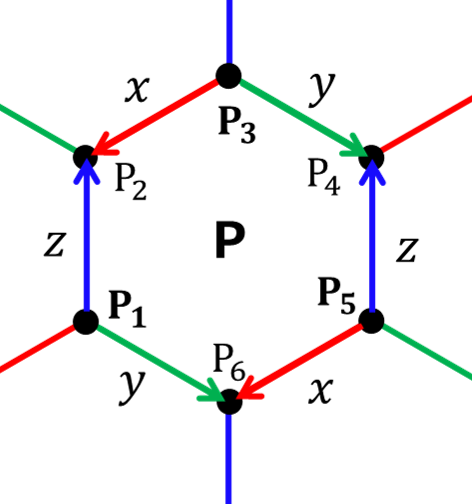
\includegraphics[width=5.0cm]{fig_kitaev/kitaev_pla.png} \\
\caption{(a)サイト$j$に対する結合.赤,緑,青はそれぞれ,$x$, $y$, $z$-interactionを表している.(b)Kitaev 模型を定義する六角格子 (honeycomb lattice).
(c)副格子.下をA-副格子,上をb-副格子と呼び,A-副格子のサイトに対応するindexを$i$とする.}
\label{fig:schematic1}
\end{figure}\begin{figure}[h]
\centering
		%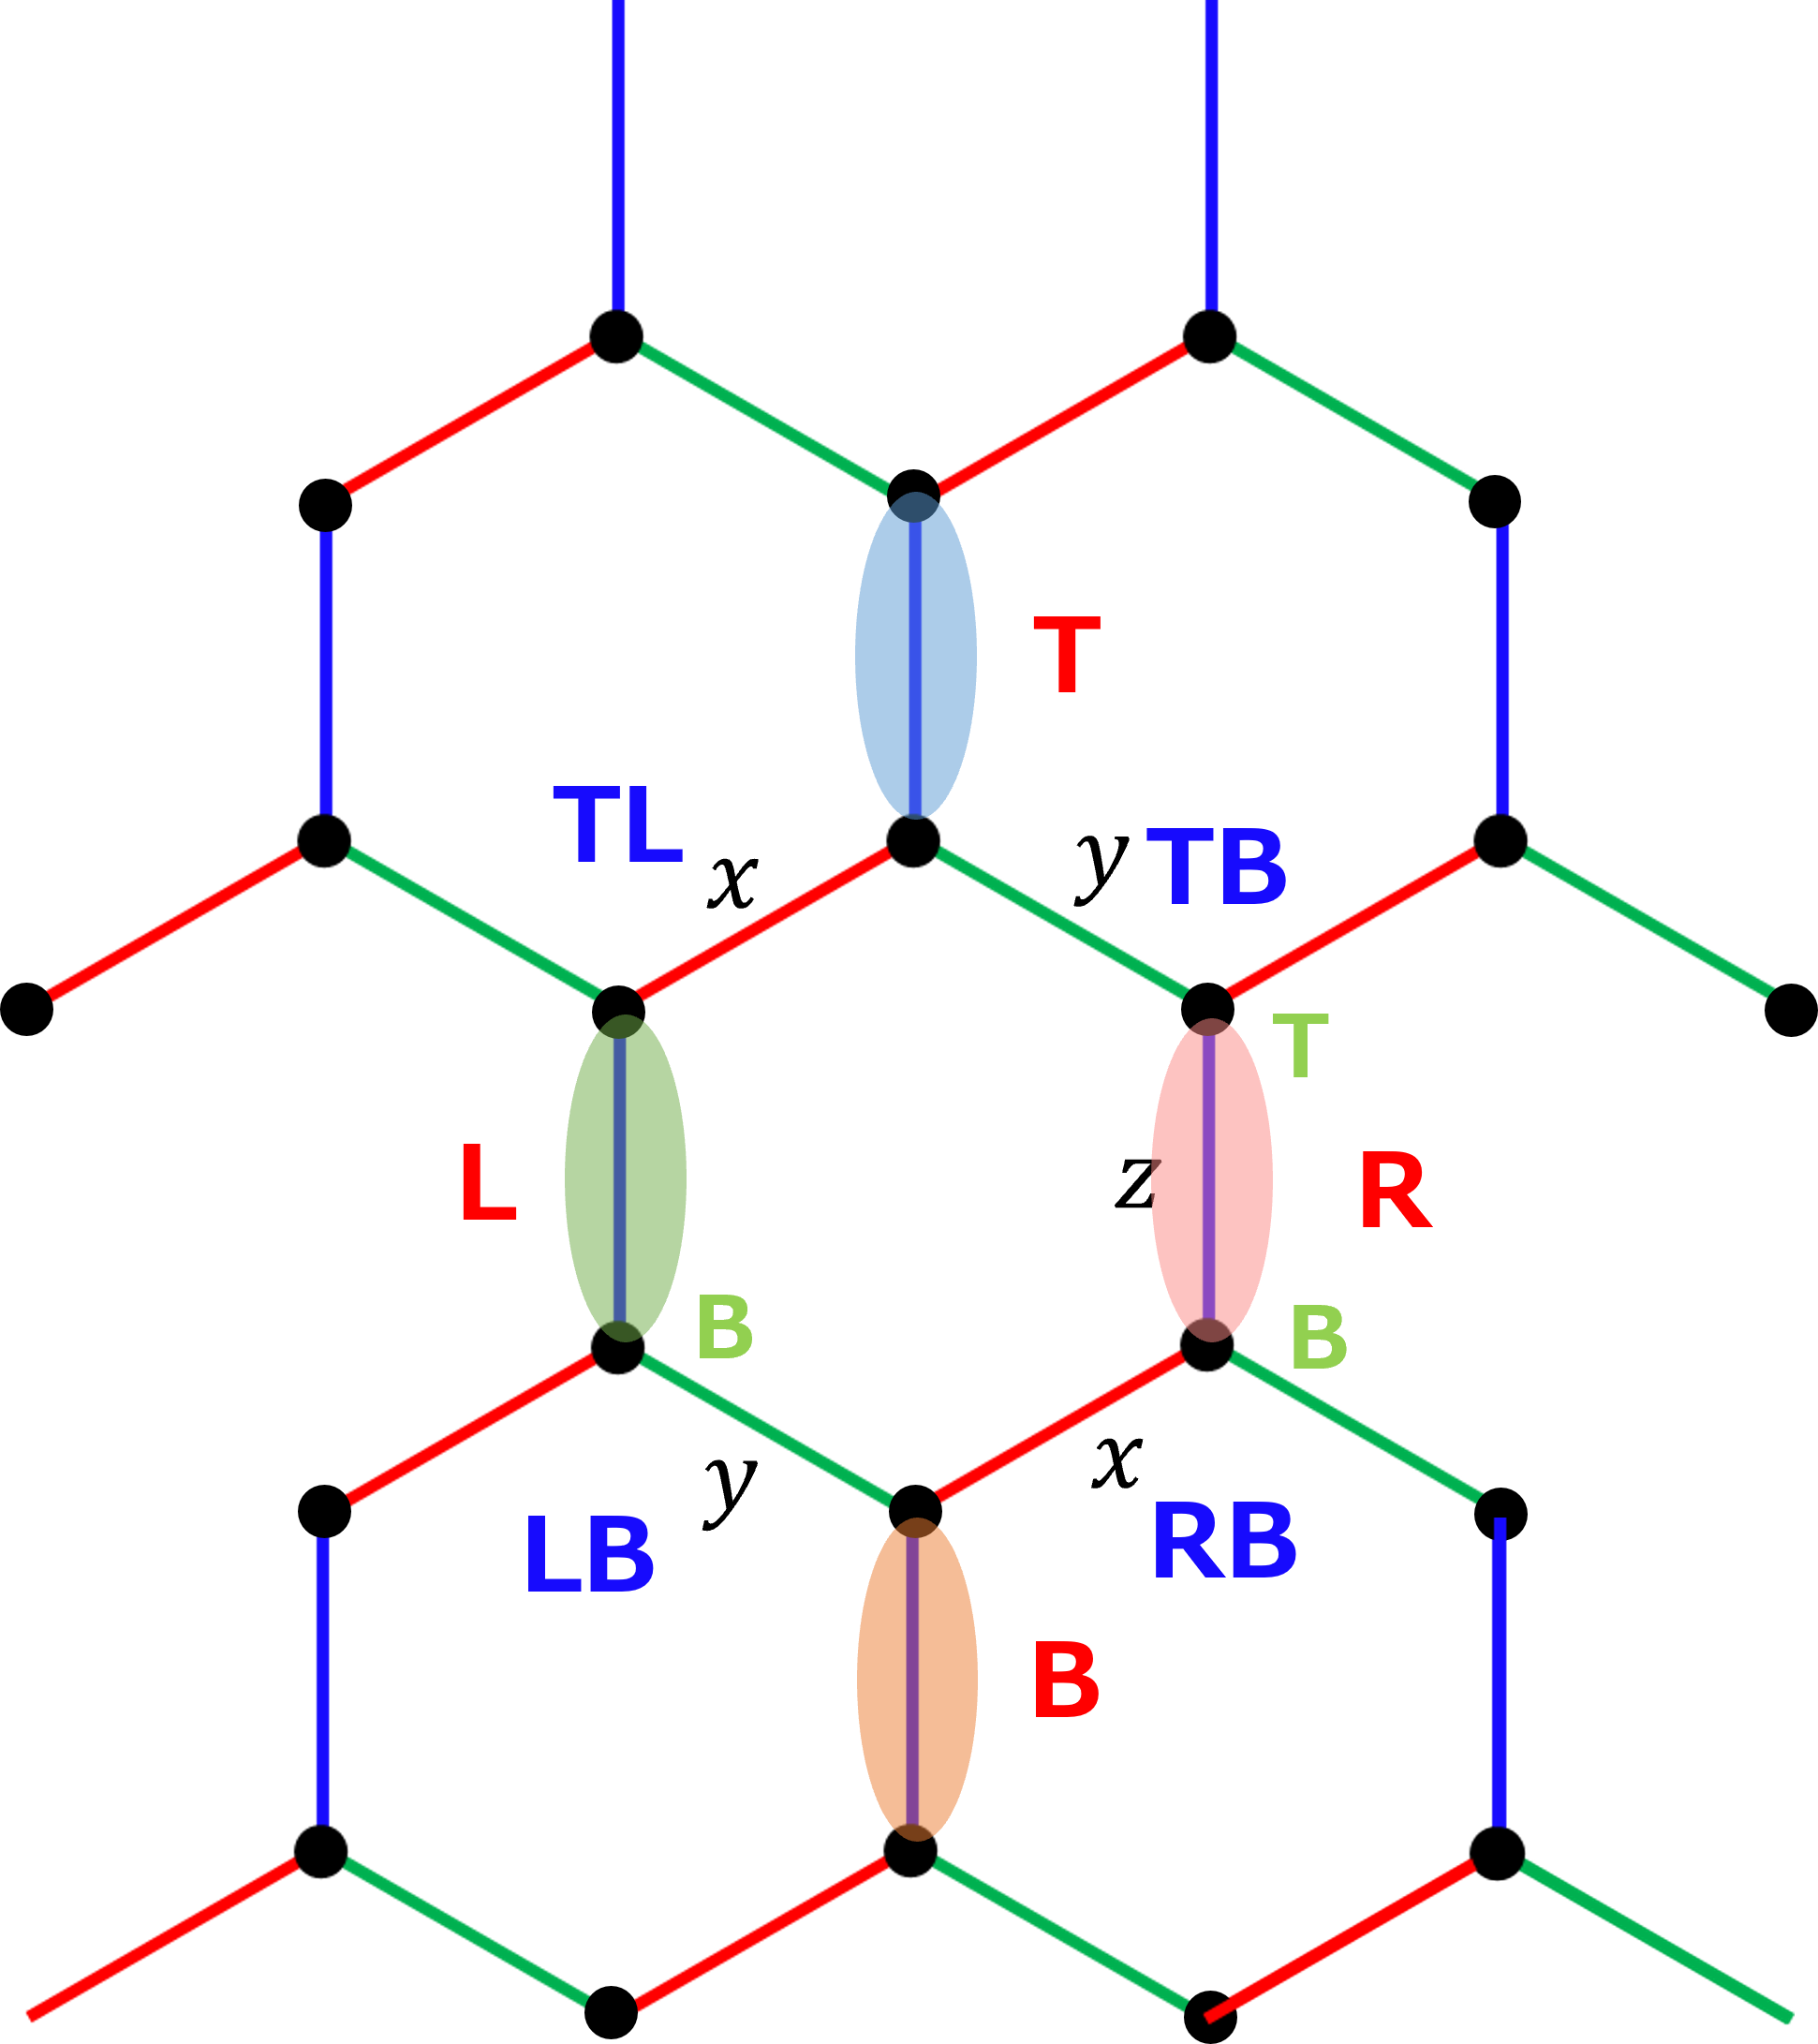
\includegraphics[width=6.0cm]{fig_kitaev/kitaev_pla2.png} \\
\caption{(a)サイト$j$に対する結合.赤,緑,青はそれぞれ,$x$, $y$, $z$-interactionを表している.(b)Kitaev 模型を定義する六角格子 (honeycomb lattice).
(c)副格子.下をA-副格子,上をb-副格子と呼び,A-副格子のサイトに対応するindexを$i$とする.}
\label{fig:schematic1}
\end{figure}

\subsection{基底状態の相図}

\section*{7th, October, 2022}
\section{Toric code limit}
\subsection{異方的極限の有効ハミルトニアン}

\subsection{低エネルギー有効模型}


\subsection{Toric code 模型への帰着}
\begin{figure}[h]
\centering
		%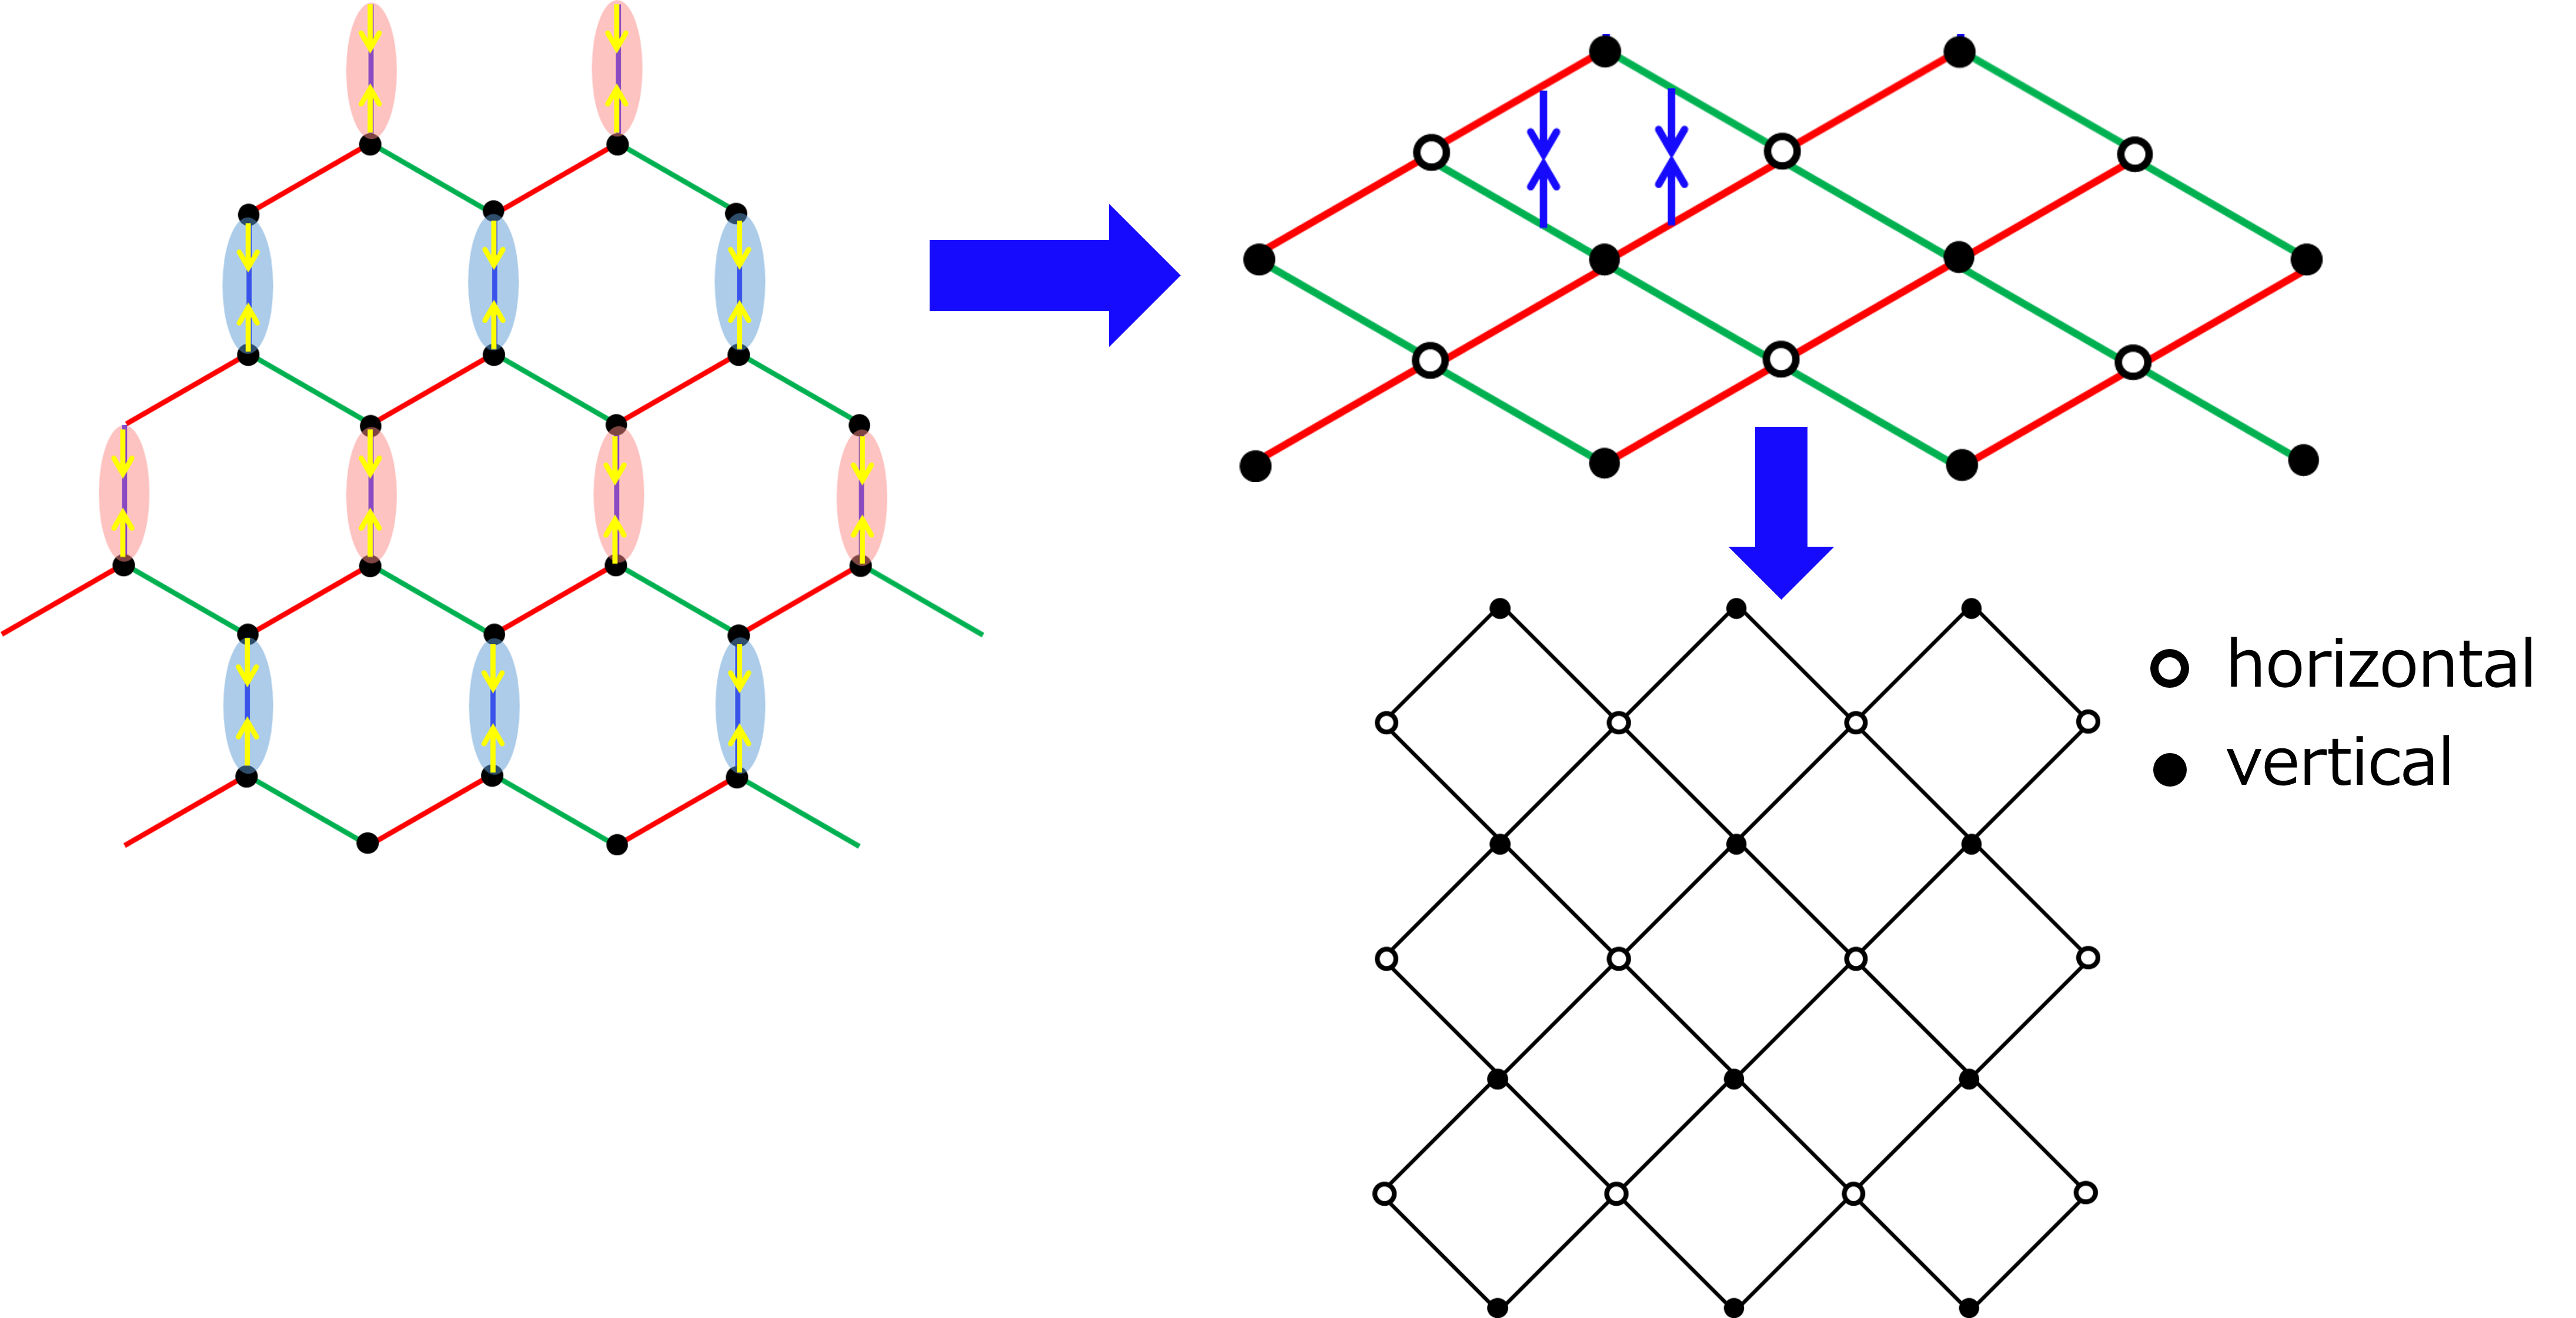
\includegraphics[width=18.0cm]{fig_toric/kitaev_to_toric.png} \\
\caption{(a)サイト$j$に対する結合.赤,緑,青はそれぞれ,$x$, $y$, $z$-interactionを表している.(b)Kitaev 模型を定義する六角格子 (honeycomb lattice).
(c)副格子.下をA-副格子,上をb-副格子と呼び,A-副格子のサイトに対応するindexを$i$とする.}
\label{fig:schematic1}
\end{figure}


\begin{figure}[h]
\centering
		%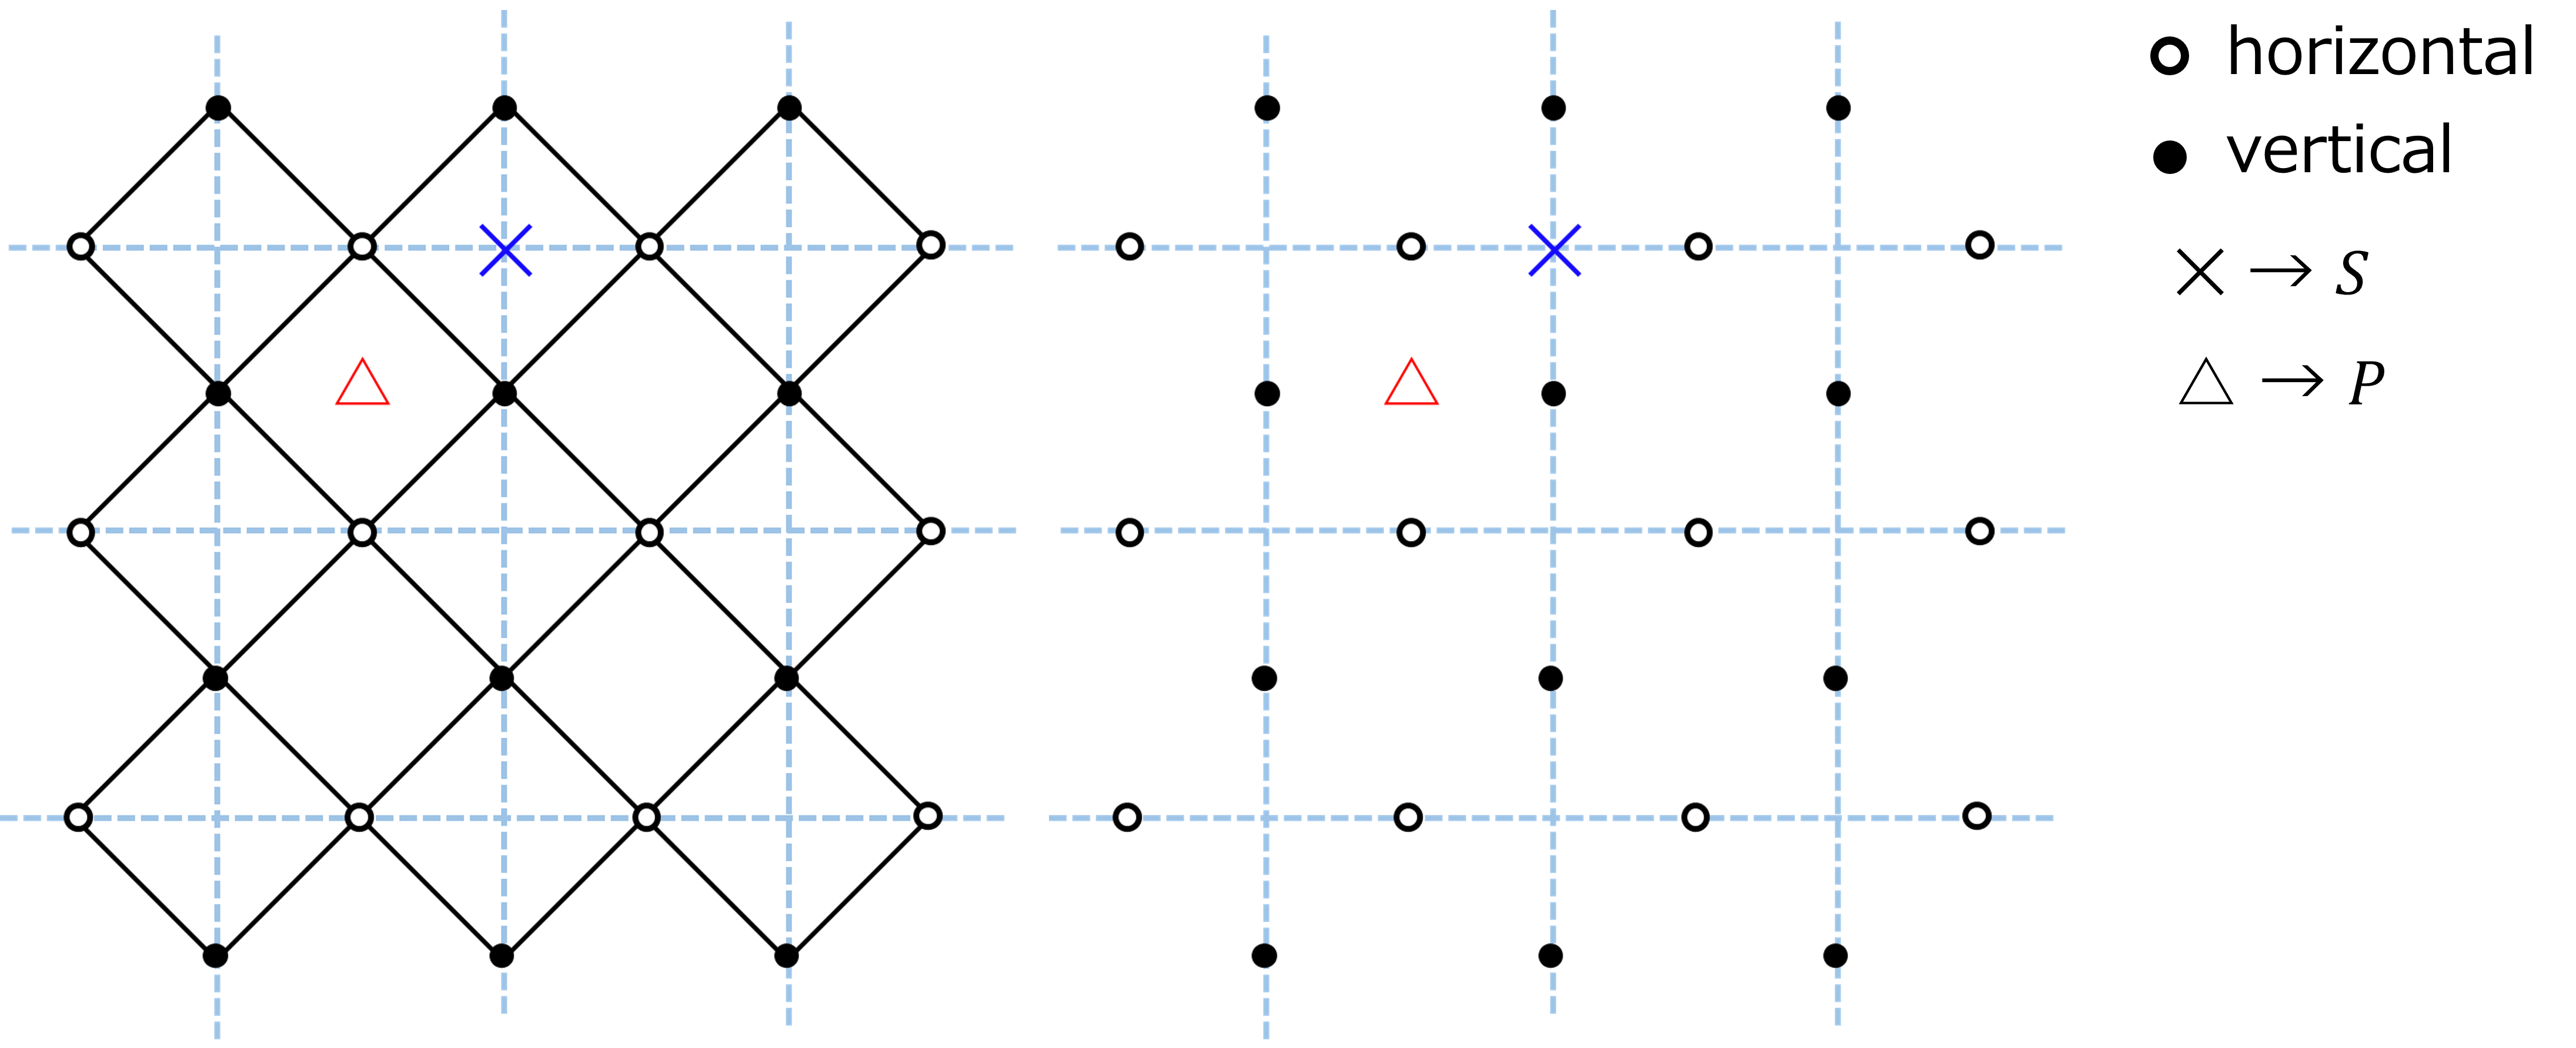
\includegraphics[width=18.0cm]{fig_toric/toric1.png} \\
\caption{(a)サイト$j$に対する結合.赤,緑,青はそれぞれ,$x$, $y$, $z$-interactionを表している.(b)Kitaev 模型を定義する六角格子 (honeycomb lattice).
(c)副格子.下をA-副格子,上をb-副格子と呼び,A-副格子のサイトに対応するindexを$i$とする.}
\label{fig:schematic1}
\end{figure}



\section*{14th, October, 2022}
\section{Toric code model}
\begin{figure}[h]
\centering
		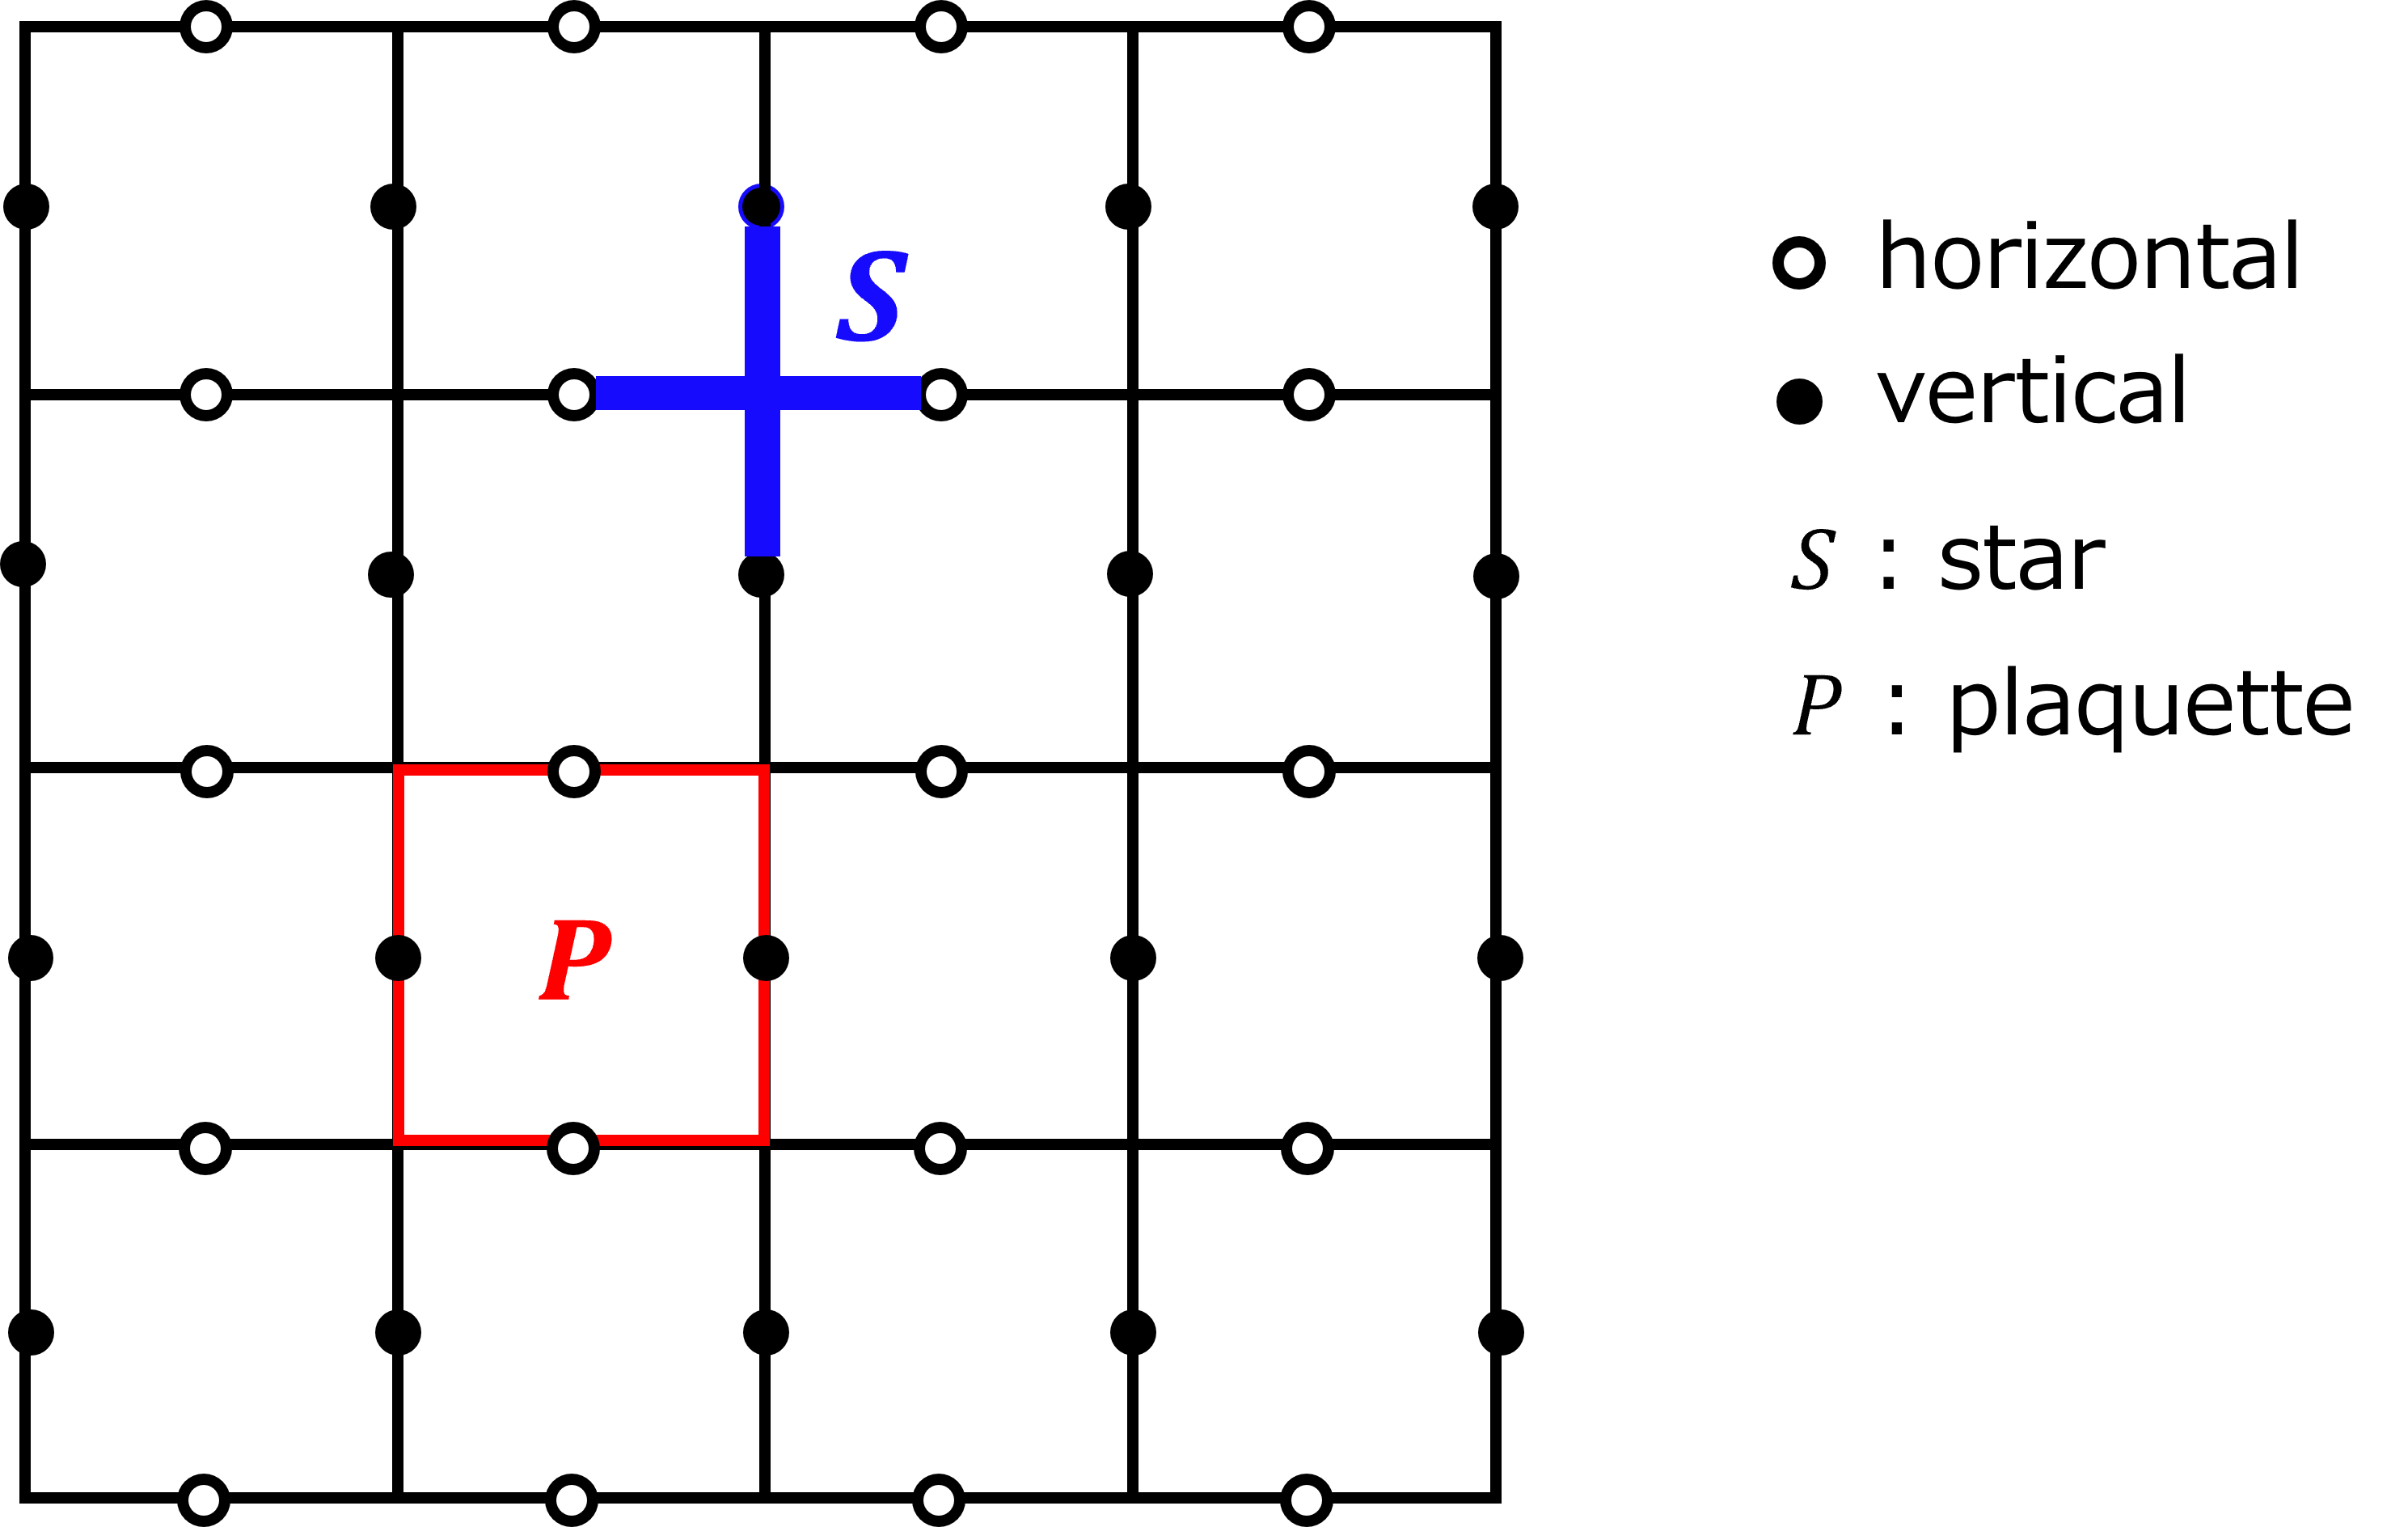
\includegraphics[width=10.0cm]{fig_toric/toric2.png} \\
\caption{(a)サイト$j$に対する結合.赤,緑,青はそれぞれ,$x$, $y$, $z$-interactionを表している.(b)Kitaev 模型を定義する六角格子 (honeycomb lattice).
(c)副格子.下をA-副格子,上をb-副格子と呼び,A-副格子のサイトに対応するindexを$i$とする.}
\label{fig:schematic1}
\end{figure}
\begin{equation}
    \hat{H}_{\rm{TC}} = -\lambda_s \sum_{s}\hat{A}_s - \lambda_p \sum_p \hat{B}_p
    =\hat{H}_{s} + \hat{H}_p
\end{equation}
\begin{align}
    \hat{A}_s 
    &= \hat{\sigma}_{s_1}^{z} \hat{\sigma}_{s_2}^{z} \hat{\sigma}_{s_3}^{z} \hat{\sigma}_{s_4}^{z}
    =\prod_{i\in s}\hat{\sigma}^{z}_{s_i}\\[10pt]
    \hat{B}_p
    &= \hat{\sigma}_{p_1}^{x} \hat{\sigma}_{p_2}^{x} \hat{\sigma}_{p_3}^{x} \hat{\sigma}_{p_4}^{x}
    =\prod_{i\in p}\hat{\sigma}^{x}_{p_i}
\end{align}
ここで,$j\in s$はstar(vertex) $s$に隣接するedgeを,$j \in p$はplaquetteに含まれるedgeを表す.

\subsection{$\hat{A}_s$, $\hat{B}_p$の性質}
\subsection*{性質1}$\hat{A}_s$, $\hat{B}_p$は全て可換である.$\hat{A}_s$どうし,$\hat{B}_p$
どうしは互いに可換であることは自明である.(単位演算子との可換性だから)

$\hat{A}_s$と$\hat{B}_p$が共有辺を持たない場合も可換であることは自明である.$\hat{A}_s$と$\hat{B}_p$が偶数個のサイトを共有するとき,Puli演算子の反交換関係$\hat{\sigma}^{z}\hat{\sigma}^{x}=-\hat{\sigma}^{x}\hat{\sigma}^{z}$より,$\hat{A}_s$と$\hat{B}_p$は可換であることがわかる:
\begin{equation}
    [\hat{A}_s,\ \hat{B}_p] = 0
\end{equation}
\paragraph{例}
可換性が非自明な例として,fig.~\ref{}の場合を考えてみよう.このとき,
\begin{align}
     \hat{A}_s 
     &= \hat{\sigma}^{z}_1\hat{\sigma}^{z}_2\hat{\sigma}^{z}_3\hat{\sigma}^{z}_4\\[10pt]
    \hat{B}_p
    &= \hat{\sigma}^{x}_1\hat{\sigma}^{x}_4\hat{\sigma}^{x}_5\hat{\sigma}^{x}_6
\end{align}
このとき,$\hat{A}_s$と$\hat{B}_p$はサイト1と4を共有する.Puli演算子の反交換関係$\hat{\sigma}^{z}\hat{\sigma}^{x}=-\hat{\sigma}^{x}\hat{\sigma}^{z}$より,
\begin{align}
     \hat{A}_s \hat{B}_p
     &= \hat{\sigma}^{z}_1\hat{\sigma}^{z}_2\hat{\sigma}^{z}_3\hat{\sigma}^{z}_4\ 
     \hat{\sigma}^{x}_1\hat{\sigma}^{x}_4\hat{\sigma}^{x}_5\hat{\sigma}^{x}_6\nn[10pt]
     &= \hat{\sigma}^{z}_1\hat{\sigma}^{x}_1
     \hat{\sigma}^{z}_2\hat{\sigma}^{z}_3\hat{\sigma}^{z}_4\hat{\sigma}^{x}_4
     \hat{\sigma}^{x}_5\hat{\sigma}^{x}_6\nn[10pt]
     &= (-1)^2\hat{\sigma}^{x}_1\hat{\sigma}^{z}_1
     \hat{\sigma}^{z}_2\hat{\sigma}^{z}_3
     \hat{\sigma}^{x}_4\hat{\sigma}^{z}_4
     \hat{\sigma}^{x}_5\hat{\sigma}^{x}_6\nn[10pt]
     &=\hat{\sigma}^{x}_1\hat{\sigma}^{x}_4
     \hat{\sigma}^{x}_5\hat{\sigma}^{x}_6\ 
     \hat{\sigma}^{z}_1
     \hat{\sigma}^{z}_2\hat{\sigma}^{z}_3
     \hat{\sigma}^{z}_4
     \nn[10pt]
     &=\hat{B}_p \hat{A}_s 
\end{align}

\subsection*{性質2}$\hat{A}_s$, $\hat{B}_p$の固有値は$\pm1$.次のように示せる:
\begin{equation}
    (\hat{A}_s)^2 = (\hat{B}_p)^2 = 1
\end{equation}


\subsection{基底状態}
$\hat{A}_s$と$\hat{B}_p$は可換なので同時に対角化可能.

$\hat{A}_s$と$\hat{B}_p$が同時対角化可能ならば,全ての$\hat{A}_s$, $\hat{B}_p$に対して固有値$+1$をもつ同時固有状態が,もしも存在すれば,基底状態を作ることができる.

そこで,$\hat{A}_s$と$\hat{B}_p$の固有状態について調べることにする.
\subsubsection{$\hat{A}_s$の固有状態}
$\hat{\sigma}^{z}$を対角化する基底を用いる.ここで,すべてのスピンが上向きの状態を考える:$\uparrow \downarrow$
\begin{equation}
    \ket{\bar{1}} = \ket{\uparrow\uparrow\cdots\uparrow}
\end{equation}
このとき,
\begin{equation}
    \hat{A}_s \ket{\bar{1}} = +1\ket{\bar{1}},\ \ \ \text{for all}\  v
\end{equation}
つまり,$\ket{\bar{1}}$は$\hat{A}_s$の固有状態であり,その固有値は$+1$となる.


\subsubsection{$\hat{B}_p$の固有状態}
次に,
\begin{equation}
    \ket{\Psi} 
    = \Biggl\{
    \prod_{p}(1 + \hat{B}_p)
    \Biggr\}\ket{\bar{1}}
\end{equation}
を考えてみる.$\hat{B}_p$どうしは可換,$\hat{B}_p(1 + \hat{B}_p) = 1 + \hat{B}_p$より,
\begin{equation}
    \hat{B}_p\ket{\Psi} 
    = \hat{B}_p\Biggl\{
    \prod_{p}(1 + \hat{B}_p)
    \Biggr\}\ket{\bar{1}}
    = \Biggl\{
    \prod_{p}\hat{B}_p(1 + \hat{B}_p)
    \Biggr\}\ket{\bar{1}}
    = \Biggl\{
    \prod_{p}(1 + \hat{B}_p)
    \Biggr\}\ket{\bar{1}}
    =+1\ket{\Psi}
\end{equation}
よって,$\ket{\Psi}$は$\hat{B}_p$の固有状態であり,その固有値は$+1$である.この状態は量子情報の文脈で,surface code状態とも呼ばれている.

性質1より,$\hat{A}_s (1 + \hat{B}_p) =  (\hat{A}_s + \hat{A}_s\hat{B}_p) = (\hat{A}_s + \hat{B}_p \hat{A}_s) = (1 + \hat{B}_p )\hat{A}_s$となるから,
\begin{equation}
    \hat{A}_s \ket{\Psi} 
    =  \hat{A}_s\Biggl\{
    \prod_{p}(1 + \hat{B}_p)
    \Biggr\}\ket{\bar{1}}
    =  \Biggl\{
    \prod_{p}(1 + \hat{B}_p)
    \Biggr\}\hat{A}_s\ket{\bar{1}}
    =\Biggl\{
    \prod_{p}(1 + \hat{B}_p)
    \Biggr\}\ket{\bar{1}}
    =\ket{\Psi}
\end{equation}
ここで,$\hat{A}_s\ket{\bar{1}} = \ket{\bar{1}}$を用いた.よって,$\ket{\Psi}$は$\hat{A}_s$と$\hat{B}_p$, $(\forall s, p)$の固有値$+1$に属する同時固有状態であるといえる.


\subsection{トポロジカル縮退}
\subsubsection{別の基底状態}



\subsection{励起状態}




\section{Stabilizer state}

\bibliographystyle{unsrt}%参考文bibliographystyle献出力スタイル
\bibliography{myrefs}
\end{document}


\section{simulation of toric code}
The Ground State
----------------

 While individual X and Z operators do not commute with each other, the X Group and Z Group operators
 do:

 .. math::

      [S_s, P_p] = 0.

 Since they commute, the wavefunction can be an eigenstate of each group operator independently. To minimize
 the energy of the Hamiltonian on the system as a whole, we can minimize the contribution of each group operator.
 Due to the negative coefficients in the Hamiltonian, we need to maximize the
 expectation value of each operator.
 The maximum possible expectation value for each operator is :math:`+1`. We can turn this
 into a constraint on our ground state:

 .. math::

       S_s |G \rangle = +1 |G \rangle \qquad \qquad P_p | G \rangle = +1 |G\rangle.

 The wavefunction

 .. math::

    | G \rangle =  \prod_{p} \frac{\mathbb{I} + P_p}{\sqrt{2}} |00\dots 0\rangle = \prod_{p} U_p |00\dots 0 \rangle,

 where :math:`P_p` (plaquette) denotes an X Group operator, is such a state.

 .. note::

    To check your understanding, confirm that this ground state obeys the constraints using pen and paper.

 :math:`|G \rangle` contains a product of unitaries :math:`U_p`. If we can figure out how to apply a single
 :math:`U_p` using a quantum computer's operations, we can apply that decomposition
 for every :math:`p` in the product.

 To better understand how to decompose :math:`U_p`, let’s write
 it concretely for a single group of four qubits:

 .. math::
    U |0000 \rangle =
    \frac{\left(\mathbb{I} + X_1 X_2 X_3 X_4 \right)}{\sqrt{2}} |0000 \rangle
    = \frac{1}{\sqrt{2}} \left( |0000\rangle + |1111\rangle \right).

 This `generalized GHZ state <https://en.wikipedia.org/wiki/Greenberger–Horne–Zeilinger_state>`__
 can be prepared with a Hadamard and 3 CNOT
 gates:

 .. figure:: ../demonstrations/toric_code/generalized_ghz_draw.png
     :align: center
     :width: 50%

 This decomposition for :math:`U_p` holds only when the initial Hadamard
 qubit begins in the :math:`|0\rangle` state, so we need to be careful in
 the choice of the Hadamard's qubit. This restriction is
 why we rotated the order for a single X Group on the right border
 earlier.

 We will also not need to prepare the final X Group that contains the
 four edges of the lattice.

 Now let’s actually put these together into a circuit!





